 \documentclass[luatex,onecolumn,showpacs,aps,preprint,prb,amsfonts,amsmath,amssymb,floatfix,groupedaddress, longbibliography]{revtex4-2} 
	\def\papertitle{Paper Title}
	\def\authors{Author Name}
	\def\journal{}
	\def\doi{}

%%%% START preamble.tex
\usepackage[includeheadfoot,top=20mm, bottom=20mm, footskip=2.5cm]{geometry}

% Typography
\usepackage[T1]{fontenc}
\usepackage{times}
%\usepackage{mathptmx} % math also in times font
\usepackage{amssymb,amsmath}
\usepackage{microtype}
\usepackage[utf8]{inputenc}

% Misc
\usepackage{graphicx}
\usepackage[colorlinks=true,citecolor=blue,linkcolor=blue,urlcolor=blue]{hyperref}
\usepackage{soul} % Highlight using \hl{}
\usepackage{lipsum}

% Table
\usepackage{adjustbox} % center large tables across textwidth by surrounding tabular with \begin{adjustbox}{center}
\renewcommand{\arraystretch}{1.5} % enlarge spacing between rows
\usepackage{caption} 
\captionsetup[table]{skip=10pt} % enlarge spacing between caption and table

% Section styles

\usepackage{titlesec}
\titleformat{\section}{\normalfont\large}{\makebox[0pt][r]{\bf \thesection.\hspace{4mm}}}{0em}{\bfseries}
\titleformat{\subsection}{\normalfont}{\makebox[0pt][r]{\bf \thesubsection.\hspace{4mm}}}{0em}{\bfseries}
\titlespacing{\subsection}{0em}{1em}{-0.3em} % left before after

% Paragraph styles

\setlength{\parskip}{0.6\baselineskip}
\setlength{\parindent}{0pt}

% Quotation styles

\usepackage{framed}
\let\oldquote=\quote
\let\endoldquote=\endquote
\renewenvironment{quote}{\begin{fquote}\advance\leftmargini -2.4em\begin{oldquote}}{\end{oldquote}\end{fquote}}

\usepackage{xcolor}
\newenvironment{fquote}
  {\def\FrameCommand{
	\fboxsep=0.6em % box to text padding
	\fcolorbox{black}{white}}%
	% the "2" can be changed to make the box smaller
    \MakeFramed {\advance\hsize-2\width \FrameRestore}
    \begin{minipage}{\linewidth}
  }
  {\end{minipage}\endMakeFramed}

% Table styles

\let\oldtabular=\tabular
\let\endoldtabular=\endtabular
\renewenvironment{tabular}[1]{\begin{adjustbox}{center}\begin{oldtabular}{#1}}{\end{oldtabular}\end{adjustbox}}


% Shortcuts

%% Let textbf be both, bold and italic
%\DeclareTextFontCommand{\textbf}{\bfseries\em}

%% Add RC and AR to the left of a paragraph
%\def\RC{\makebox[0pt][r]{\bf RC:\hspace{4mm}}}
%\def\AR{\makebox[0pt][r]{AR:\hspace{4mm}}}

%% Define that \RC and \AR should start and format the whole paragraph 
\usepackage{suffix}
\long\def\RC#1\par{\makebox[0pt][r]{\bf RC:\hspace{4mm}}\textbf{\textit{#1}}\par} %\RC
\WithSuffix\long\def\RC*#1\par{\textbf{\textit{#1}}\par} %\RC*
% \long\def\AR#1\par{\makebox[0pt][r]{AR:\hspace{10pt}}\textit{#1}\par} %\AR
\long\def\AR#1\par{\makebox[0pt][r]{AR:\hspace{10pt}}#1\par} %\AR
\WithSuffix\long\def\AR*#1\par{\textit{#1}\par} %\AR*

%%%
%DIF PREAMBLE EXTENSION ADDED BY LATEXDIFF
%DIF UNDERLINE PREAMBLE %DIF PREAMBLE
\RequirePackage[normalem]{ulem} %DIF PREAMBLE
\RequirePackage{color}\definecolor{RED}{rgb}{1,0,0}\definecolor{BLUE}{rgb}{0,0,1} %DIF PREAMBLE
\providecommand{\DIFadd}[1]{{\protect\color{blue}\uwave{#1}}} %DIF PREAMBLE
\providecommand{\DIFdel}[1]{{\protect\color{red}\sout{#1}}}                      %DIF PREAMBLE
%DIF SAFE PREAMBLE %DIF PREAMBLE
\providecommand{\DIFaddbegin}{} %DIF PREAMBLE
\providecommand{\DIFaddend}{} %DIF PREAMBLE
\providecommand{\DIFdelbegin}{} %DIF PREAMBLE
\providecommand{\DIFdelend}{} %DIF PREAMBLE
%DIF FLOATSAFE PREAMBLE %DIF PREAMBLE
\providecommand{\DIFaddFL}[1]{\DIFadd{#1}} %DIF PREAMBLE
\providecommand{\DIFdelFL}[1]{\DIFdel{#1}} %DIF PREAMBLE
\providecommand{\DIFaddbeginFL}{} %DIF PREAMBLE
\providecommand{\DIFaddendFL}{} %DIF PREAMBLE
\providecommand{\DIFdelbeginFL}{} %DIF PREAMBLE
\providecommand{\DIFdelendFL}{} %DIF PREAMBLE
%DIF END PREAMBLE EXTENSION ADDED BY LATEXDIFF

% Define title defaults if not defined by user
\providecommand{\lettertitle}{Author Response to Reviews of}
\providecommand{\papertitle}{Title}
\providecommand{\authors}{Authors}
\providecommand{\journal}{Journal}
% \providecommand{\doi}{--}


% others ...
\usepackage{siunitx}
\usepackage{standalone}
\usepackage{mhchem}
\usepackage{graphicx}

% 
\renewcommand{\thefigure}{A\arabic{figure}}
\renewcommand{\thetable}{A\arabic{table}}
% \setcounter{figure}{0}
% \setcounter{table}{0}


\usepackage{cleveref}
\crefname{figure}{Fig.}{Fig.}
\crefname{table}{Table}{Table}


\begin{document}

% Make title
{\Large\bf \lettertitle}\\[1em]
{\huge \papertitle}\\[1em]
{\authors}\\
% {\it \journal, }\texttt{doi:\doi}\\
\hrule

% Legend
\hfill {\bfseries RC:} \textbf{\textit{Reviewer Comment}},\(\quad\) AR: \emph{Author Response}, \(\quad\square\) Manuscript text

\section{Summary of Update}

\lipsum[10]

These are highlighted by red in the attached highlighted manuscript except for minor grammatical corrections.

\begin{itemize}
  \item The abstract has benn slightly modified for more accurate description.
  \item We have performed new calculations, and have added related results and discussions. 
  \item Figure. 4 was wrong in the original version, and we replaced it with correct one.
  \item Some minor corrections have been made to improve readability and clarity.
\end{itemize}


\section{The First Referee}

\subsection{General comment}

\RC \lipsum[1]

\AR We sincerely appreciate the referee’s supportive and insightful comments on our manuscript. We believe this manuscript will interest many researchers as it discusses hogehoge. Following the suggestions of the referee, we have amended the manuscript appropriately. We provided the point-by-point responses to the referee’s comments/questions below:

\subsection{\#1 Question summary}

\RC \lipsum[1]

\AR \lipsum[1]

\begin{quote}
\lipsum[2] \DIFadd{ADD THIS COMMENT~\cite{abrahams1971Rutile}.} \lipsum[2] ...
\end{quote}


\subsection{\#2 Question Summary}

\RC \lipsum[1]

\AR  \lipsum[1]

\begin{figure}[htb]
\centering
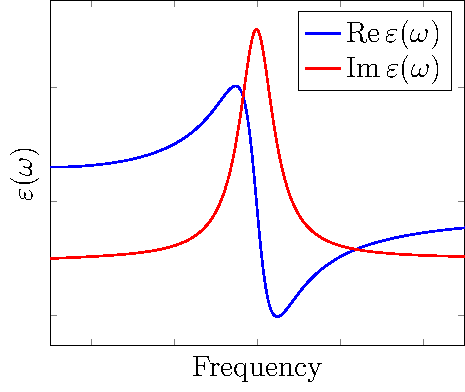
\includegraphics[]{../manuscript/figures/fig01/fig01.pdf}
\caption{Fig caption}
\label{fig:01}
\end{figure}

\lipsum[1]

\begin{table}[t] 
\centering
\caption{Table caption}
\includestandalone[mode=tex]{../manuscript/figures/table01/table01}
\label{table:01}
\end{table}

\lipsum[1]

\begin{quote}
\lipsum[2] \DIFadd{ADD THIS LINE.} \DIFdel{REMOVE THIS LINE.} \lipsum[2] ...
\end{quote}


\newpage
\section{The Second Referee}

\subsection{General Comment}

\RC \lipsum[1]

\AR \lipsum[1]

\subsection{\#1 question summary}

\RC \lipsum[1]

\AR \lipsum[1]

\begin{figure}[tb] 
\centering
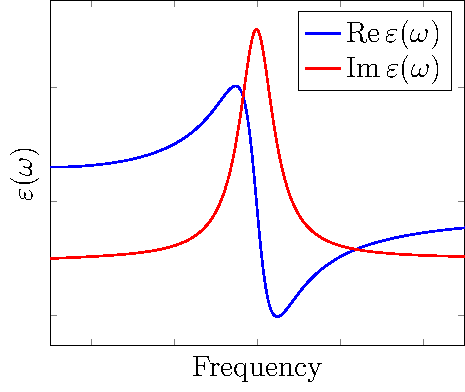
\includegraphics[]{../manuscript/figures/fig01/fig01.pdf}
\caption{Fig caption}
\label{fig:02}
\end{figure}

Since we did not include the explanation, we added the following sentence.

 \begin{quote}
\lipsum[1] \DIFadd{ADD THIS LINE.}...
\end{quote}


\subsection{\#2 Question summary}

\RC \lipsum[1]

\AR  \lipsum[1]

\begin{quote}
\DIFadd{ADD THIS LINE.} \lipsum[1]...
\end{quote}

% references(bibtex)

 \bibliographystyle{apsrev4-2}
 \bibliography{../manuscript/references/ref.bib}

\end{document}
